% AER-Article.tex for AEA last revised 22 June 2011
\documentclass[AER]{AEA}

% The mathtime package uses a Times font instead of Computer Modern.
% Uncomment the line below if you wish to use the mathtime package:
%\usepackage[cmbold]{mathtime}
% Note that miktex, by default, configures the mathtime package to use commercial fonts
% which you may not have. If you would like to use mathtime but you are seeing error
% messages about missing fonts (mtex.pfb, mtsy.pfb, or rmtmi.pfb) then please see
% the technical support document at http://www.aeaweb.org/templates/technical_support.pdf
% for instructions on fixing this problem.

% Note: you may use either harvard or natbib (but not both) to provide a wider
% variety of citation commands than latex supports natively. See below.

% Uncomment the next line to use the natbib package with bibtex
\usepackage{natbib}

% Uncomment the next line to use the harvard package with bibtex
%\usepackage[abbr]{harvard}

% This command determines the leading (vertical space between lines) in draft mode
% with 1.5 corresponding to "double" spacing.
\draftSpacing{1.5}

% Pandoc syntax highlighting
\usepackage{color}
\usepackage{fancyvrb}
\newcommand{\VerbBar}{|}
\newcommand{\VERB}{\Verb[commandchars=\\\{\}]}
\DefineVerbatimEnvironment{Highlighting}{Verbatim}{commandchars=\\\{\}}
% Add ',fontsize=\small' for more characters per line
\usepackage{framed}
\definecolor{shadecolor}{RGB}{248,248,248}
\newenvironment{Shaded}{\begin{snugshade}}{\end{snugshade}}
\newcommand{\AlertTok}[1]{\textcolor[rgb]{0.94,0.16,0.16}{#1}}
\newcommand{\AnnotationTok}[1]{\textcolor[rgb]{0.56,0.35,0.01}{\textbf{\textit{#1}}}}
\newcommand{\AttributeTok}[1]{\textcolor[rgb]{0.77,0.63,0.00}{#1}}
\newcommand{\BaseNTok}[1]{\textcolor[rgb]{0.00,0.00,0.81}{#1}}
\newcommand{\BuiltInTok}[1]{#1}
\newcommand{\CharTok}[1]{\textcolor[rgb]{0.31,0.60,0.02}{#1}}
\newcommand{\CommentTok}[1]{\textcolor[rgb]{0.56,0.35,0.01}{\textit{#1}}}
\newcommand{\CommentVarTok}[1]{\textcolor[rgb]{0.56,0.35,0.01}{\textbf{\textit{#1}}}}
\newcommand{\ConstantTok}[1]{\textcolor[rgb]{0.00,0.00,0.00}{#1}}
\newcommand{\ControlFlowTok}[1]{\textcolor[rgb]{0.13,0.29,0.53}{\textbf{#1}}}
\newcommand{\DataTypeTok}[1]{\textcolor[rgb]{0.13,0.29,0.53}{#1}}
\newcommand{\DecValTok}[1]{\textcolor[rgb]{0.00,0.00,0.81}{#1}}
\newcommand{\DocumentationTok}[1]{\textcolor[rgb]{0.56,0.35,0.01}{\textbf{\textit{#1}}}}
\newcommand{\ErrorTok}[1]{\textcolor[rgb]{0.64,0.00,0.00}{\textbf{#1}}}
\newcommand{\ExtensionTok}[1]{#1}
\newcommand{\FloatTok}[1]{\textcolor[rgb]{0.00,0.00,0.81}{#1}}
\newcommand{\FunctionTok}[1]{\textcolor[rgb]{0.00,0.00,0.00}{#1}}
\newcommand{\ImportTok}[1]{#1}
\newcommand{\InformationTok}[1]{\textcolor[rgb]{0.56,0.35,0.01}{\textbf{\textit{#1}}}}
\newcommand{\KeywordTok}[1]{\textcolor[rgb]{0.13,0.29,0.53}{\textbf{#1}}}
\newcommand{\NormalTok}[1]{#1}
\newcommand{\OperatorTok}[1]{\textcolor[rgb]{0.81,0.36,0.00}{\textbf{#1}}}
\newcommand{\OtherTok}[1]{\textcolor[rgb]{0.56,0.35,0.01}{#1}}
\newcommand{\PreprocessorTok}[1]{\textcolor[rgb]{0.56,0.35,0.01}{\textit{#1}}}
\newcommand{\RegionMarkerTok}[1]{#1}
\newcommand{\SpecialCharTok}[1]{\textcolor[rgb]{0.00,0.00,0.00}{#1}}
\newcommand{\SpecialStringTok}[1]{\textcolor[rgb]{0.31,0.60,0.02}{#1}}
\newcommand{\StringTok}[1]{\textcolor[rgb]{0.31,0.60,0.02}{#1}}
\newcommand{\VariableTok}[1]{\textcolor[rgb]{0.00,0.00,0.00}{#1}}
\newcommand{\VerbatimStringTok}[1]{\textcolor[rgb]{0.31,0.60,0.02}{#1}}
\newcommand{\WarningTok}[1]{\textcolor[rgb]{0.56,0.35,0.01}{\textbf{\textit{#1}}}}

% tightlist command for lists without linebreak
\providecommand{\tightlist}{%
  \setlength{\itemsep}{0pt}\setlength{\parskip}{0pt}}



\usepackage{graphicx}
\usepackage{booktabs}

\usepackage{hyperref}

\begin{document}


\title{Global \(CO_{2}\) Emissions in 1997}
\shortTitle{What Keeling missed all these years}
% \author{Author1 and Author2\thanks{Surname1: affiliation1, address1, email1.
% Surname2: affiliation2, address2, email2. Acknowledgements}}


\author{
  Majid Maki-Nayeri\\
  Vinod Bakthavachalam\\
  D. Alex Hughes\thanks{
  Maki-Nayeri: UC Berkeley, School of
Information, \href{mailto:m\_maki@ischool.berkeley.edu}{m\_maki@ischool.berkeley.edu}.
  Bakthavachalam: UC Berkeley, School of
Information, \href{mailto:vinodb@ischool.berkeley.edu}{vinodb@ischool.berkeley.edu}.
  Hughes: , \href{mailto:dontatme@ischool.berkeley.edu}{dontatme@ischool.berkeley.edu}.
  The authors would like to thank their instructors from MIDS 271.
}
}

\date{\today}
\pubMonth{06}
\pubYear{2022}
\pubVolume{0}
\pubIssue{0}
\JEL{}
\Keywords{Replication, Modern Science}

\begin{abstract}
The year is 1997 and global attention is turning toward the consequences
of human-actions in our environmental system. The IPCC has been in
existence and studying these trends for more than ten years, and has
released its second assessment report in 1995. In this report, the IPCC
notes that the balance of the evidence suggests that human-actions play
a role in the changing climate. Although, there is little political will
to change this activity, neither have global progressive and
conservative politicians broken into clear partisan camps. Here, we
assess data from the Mona Loa observatory to describe and predict global
\(CO_{2}\) concentrations under several possible scenarios. What we
find, when we run the analysis, is going to be grim.
\end{abstract}


\maketitle

\begin{Shaded}
\begin{Highlighting}[]
\DocumentationTok{\#\# Students this file and the supporting files to create }
\DocumentationTok{\#\# the document come from the \textasciigrave{}rticles\textasciigrave{} package. }
\DocumentationTok{\#\# }
\DocumentationTok{\#\# You\textquotesingle{}re not required to write something using this template; }
\DocumentationTok{\#\# and, you might think that it hampers understanding. That\textquotesingle{}s }
\DocumentationTok{\#\# totally fine. If you would like to see other tempates, }
\DocumentationTok{\#\# you can install, the \textasciigrave{}rticles\textasciigrave{} package, and then use the}
\DocumentationTok{\#\# templates it provides. }
\DocumentationTok{\#\# install.packages(\textquotesingle{}rticles\textquotesingle{})}
\DocumentationTok{\#\# would do the trick. }
\end{Highlighting}
\end{Shaded}

Understanding a changing climate, and what it means for the earth's
inhabitants is of growing interest to the scientific and policy
community. Although, at this point in 1997 it is not entirely clear what
the consequences of this growing awareness will be, in this report we
present likely outcomes under ``business-as-usual'' scenarios. In doing
so, our hope, is to establish a series of possible futures, and, as
evidence, technology, and policy develop over the coming decades, that
we can weigh the impacts that carbon-emission reduction efforts might
take.

\hypertarget{background}{%
\section{Background}\label{background}}

\hypertarget{carbon-emissions}{%
\subsection{Carbon Emissions}\label{carbon-emissions}}

What are are carbon emissions, and why should anyone care about them? In
this section, we briefly review what is known about the relationship
between the burning of fossil fuels, atmospheric \(CO_{2}\), and the
scientific community's growing understanding of the linkage between
atmospheric \(CO_{2}\) and global average temperatures.

Blah blah blah\ldots{}

\hypertarget{measurement-and-data}{%
\section{Measurement and Data}\label{measurement-and-data}}

\hypertarget{measuring-atmospheric-carbon}{%
\subsection{Measuring Atmospheric
Carbon}\label{measuring-atmospheric-carbon}}

Crucial to forecasting levels of atmospheric carbon is reliable
measurement of this
concept.\footnote{MIDS students: Think about this, for a moment. Suppose that you were to measure atmospheric carbon directly outside a steel-foundry in Michigan. How reliable a measurement of global atmospheric carbon do you think this would be? What if that were the only measure that you had, would you still propose to write this paper? I certainly hope not.}
Several reference measurements have been proposed: Measurement 1 in
Washington, DC; Measurement 2 in Bern Switzerland \ldots{} . In this
study, we rely on \ldots{}

\hypertarget{historical-trends-in-atmospheric-carbon}{%
\subsection{Historical Trends in Atmospheric
Carbon}\label{historical-trends-in-atmospheric-carbon}}

Atmospheric carbon is plotted in \autoref{fig:carbon}, and shows some
worrying trends. Just look at how wobbly that line is. How is it
possible that we are not living in a simulation, when the lines that
plots monthly average \(CO_{2}\) looks like this?

\begin{figure}
  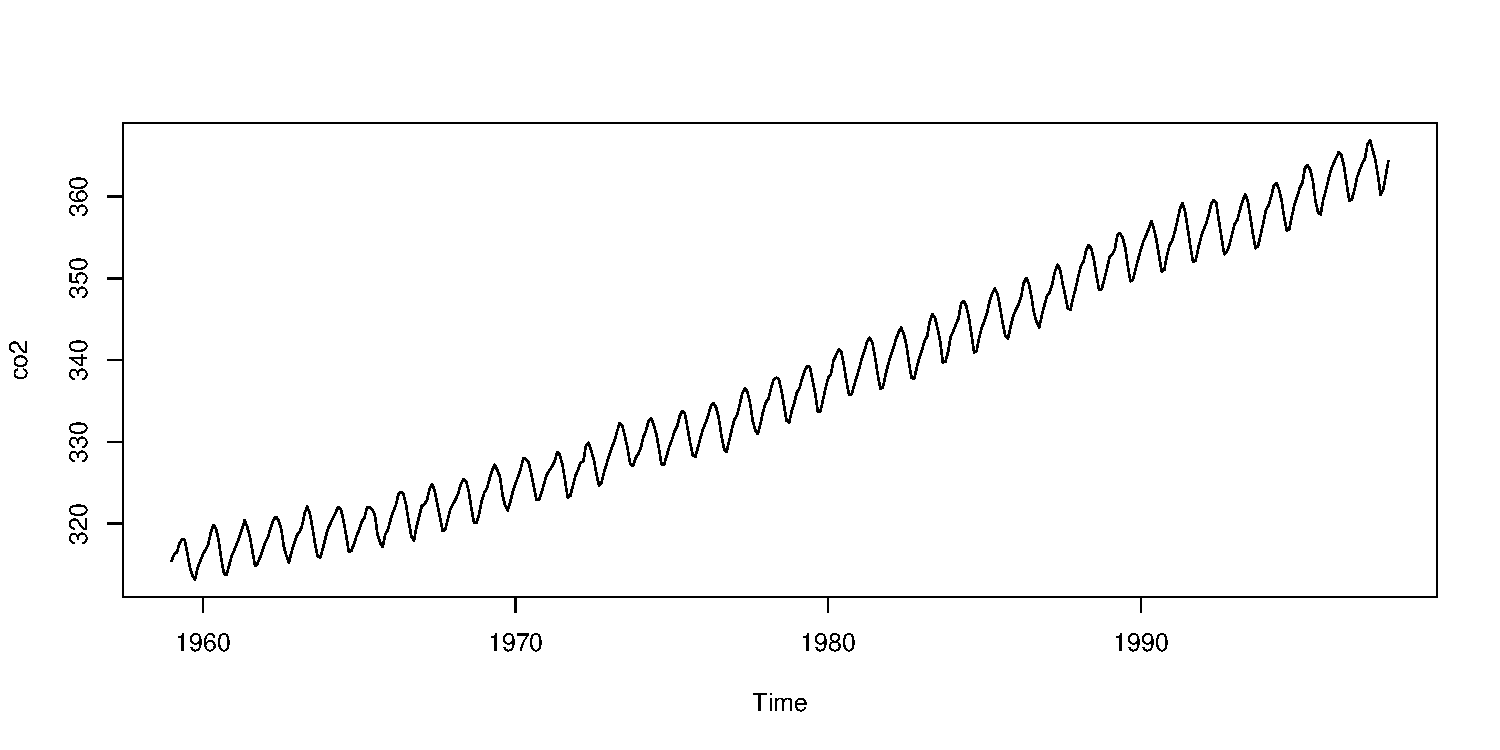
\includegraphics[width=.8\linewidth]{./figures/plot_1.pdf}
  \caption{An uncareful plot.\label{fig:carbon}}
  \begin{figurenotes}
    After giving a declarative statement about what is in the plot, it is useful to provide a very concise interpretation of what you see, or how you read the plot. It should be possible for a reader to \textit{almost} read your entire report from tables, figures, and estimated models.
  \end{figurenotes}
\end{figure}

Even more, a careful examination of \autoref{tab:table_1} suggests some
worrying trends in headings and columns.

\begin{table}
  \caption{What is happening with headers?\label{tab:table_1}}
  \begin{tabular}{lll}
    \toprule 
    & Heading 1 & Heading 2 \\
    Row 1 & 1 & 2 \\
    Row 2 & 3 & 4 \\
    \bottomrule
  \end{tabular}
  \begin{tablenotes}
    Table notes environment without optional leadin.
  \end{tablenotes}
\end{table}

\hypertarget{models-and-forecasts}{%
\section{Models and Forecasts}\label{models-and-forecasts}}

While these plots might be compelling, it is often challenging to learn
the exact nature of a time serires process from only these overview,
``time vs.~outcome'' style of plots. In this section, we present
evaluate two classes models to assess which time series model is most
appropriate to use.

\hypertarget{linear-models}{%
\subsection{Linear Models}\label{linear-models}}

To begin, we fit a model of the form:

\begin{equation}
\label{eq:one}
\text{CO}_{2} = \phi_{0} + \phi_{1} + \epsilon_{eit}
\end{equation}

which, a student of the class will immediately realize is a nonsense
model that is senseless. However, writing out the model form that you
are going to estimate makes it very clear what you're assuming about the
data generating process. It also allows you to reference what models
your forecasts are being generated from. We will be expecting such a
declaration in your reports.

We estimate best fitting parameters on this model in the following way,

\begin{Shaded}
\begin{Highlighting}[]
\NormalTok{model\_1 }\OtherTok{\textless{}{-}} \FunctionTok{lm}\NormalTok{(y }\SpecialCharTok{\textasciitilde{}}\NormalTok{ x, }\AttributeTok{data =}\NormalTok{ d)}
\end{Highlighting}
\end{Shaded}

\hypertarget{arima-models}{%
\subsection{ARIMA Models}\label{arima-models}}

Sure we also fit some ARIMA models. And talk about them.

\hypertarget{forecasts}{%
\subsection{Forecasts}\label{forecasts}}

Because we have fitted a model, we can make predictions from that model.
Our preferred model, named in \autoref{eq:one} is quite simple, and as
you might notice, does not in fact match up with the model that we have
fitted. However, from this model is is possible to reason about what the
outcomes would be if the \emph{input concept} were to be slightly ouside
of the observed data range. In particular, if \emph{input concept} were
as high as \(11\), then we would expect the \emph{output concept} to be
10.171, with a prediction interval that ranges from {[}6.546, 13.796{]}

\hypertarget{conclusions}{%
\section{Conclusions}\label{conclusions}}

What to conclude is unclear.

\bibliographystyle{aea}
\bibliography{references}

\appendix
\section{Appendix: Model Robustness}

While the most plausible model that we estimate is reported in the main,
``Modeling'' section, in this appendix to the article we examine
alternative models. Here, our intent is to provide a skeptic that does
not accept our assessment of this model as an ARIMA of order (1,2,3) an
understanding of model forecasts under alternative scenarios.


\end{document}
